% This file is part of the Open Source project 'proTironeComputatri'
% (c) 2025 Karsten Reincke (https://github.com/pro-tirone-computatri/protico.ltx)
% It is distributed under the terms of the creative commons license
% CC-BY-4.0 (= https://creativecommons.org/licenses/by/4.0/)

\selectlanguage{ngerman}

{
\usebackgroundtemplate{\includegraphics[width=\paperwidth]{\imgLf/woman-considering-1080572-pxh.png}}
\begin{frame}  
  \frametitle{Deutsch:Curriculum}

  \vspace{4cm}
  \begin{flushright}
    \textcolor{blue}{Wer bestimmt eigentlich, \\
    was in Sachen \\deutscher Schriftsprache  \\
    richtig und was falsch ist?}
  \end{flushright}
\end{frame}
}

\begin{frame}  
  \frametitle{Deutsch:Curriculum:Entscheiderinnen}
  \begin{center}
  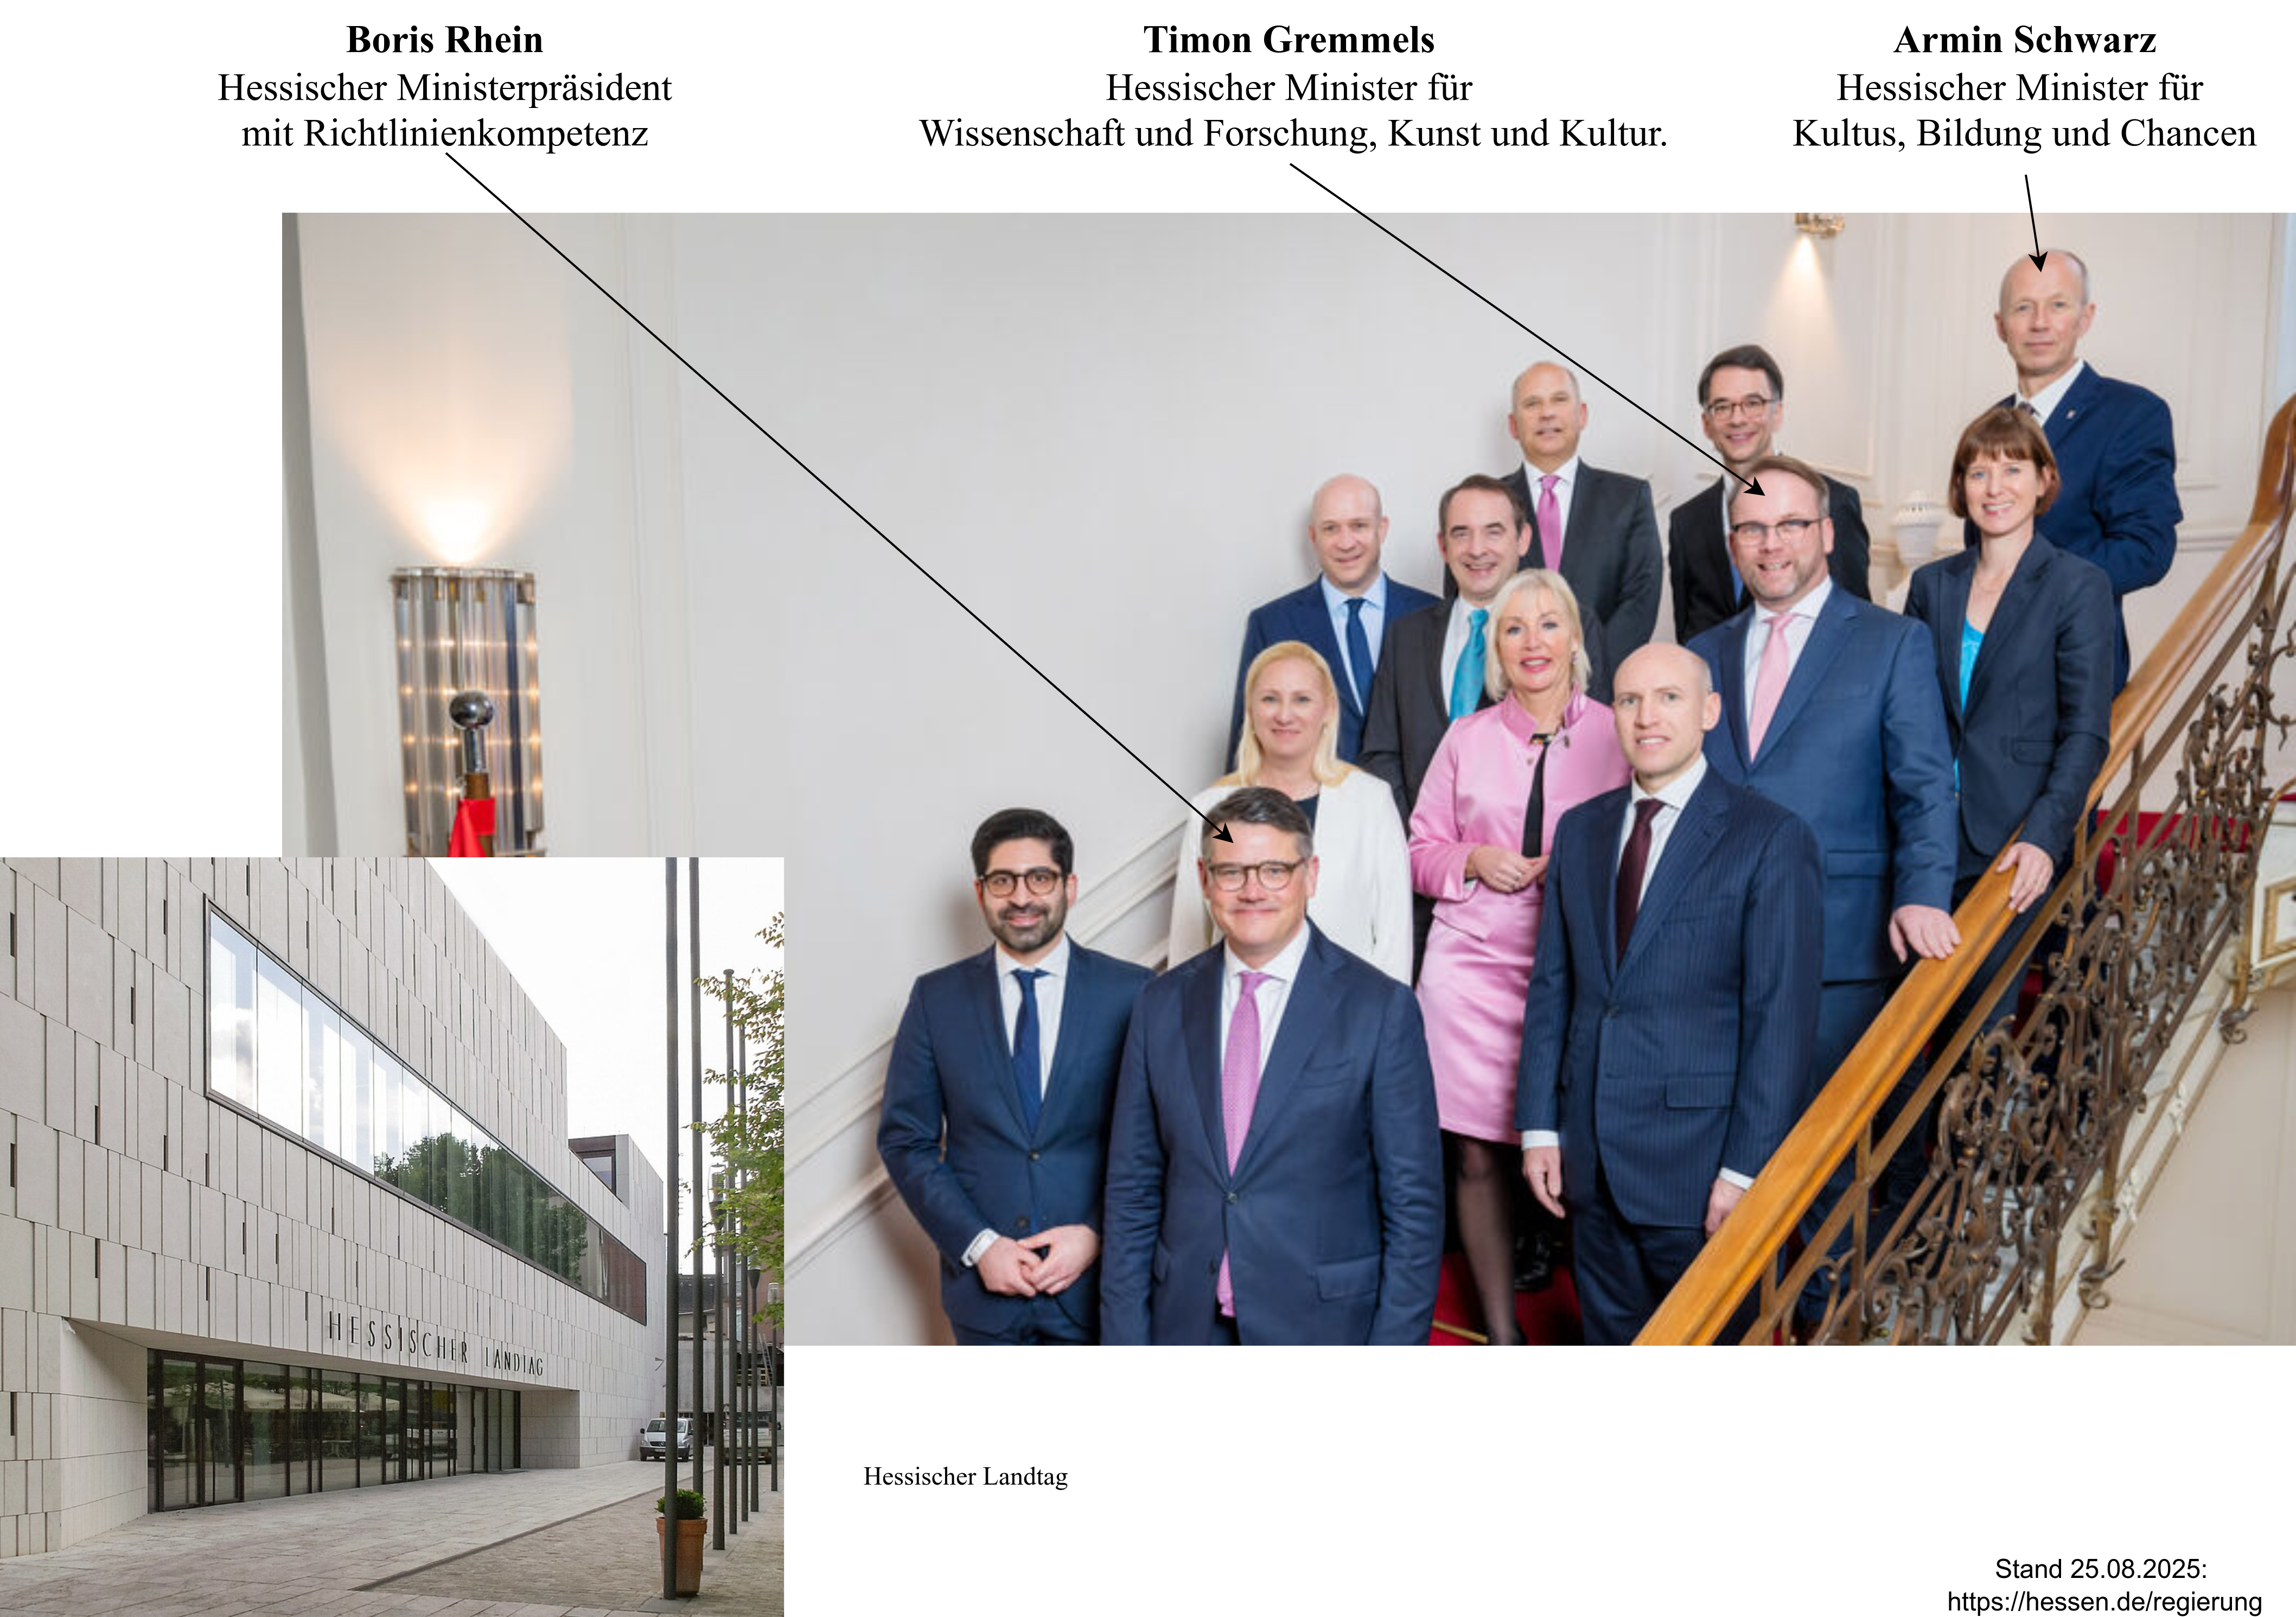
\includegraphics[width=10cm]{\imgGl/hessen-regierung.png}
  \end{center}
\end{frame}

{
\usebackgroundtemplate{\includegraphics[width=\paperwidth]{\imgLf/smartphone-4669-pxh.png}}
\begin{frame}  
  \frametitle{Deutsch:Curriculum:Entscheidungsbeispiel}

  \vspace{6cm}
  \begin{flushright}
    \textcolor{white}{Hessens neue Handyregelung!}
  \end{flushright}
\end{frame}
}

{
\usebackgroundtemplate{\includegraphics[width=\paperwidth]{\imgLf/fragmenting-759708-pxh.png}}
\begin{frame}  
  \frametitle{Deutsch:Curriculum:Fragmentierung}

  \vspace{7cm}
  \begin{flushright}
    \textcolor{magenta}{Jedes Land für sich?}
  \end{flushright}
\end{frame}
}

\begin{frame}
  \frametitle{Deutsch:Curriculum:supraförderal}
  \begin{figure}
    \includegraphics[width=11cm]{\imgGl/kmk-logo.png}
  \end{figure}
\end{frame}

\begin{frame}
  \frametitle{Deutsch:Curriculum/supranational}
  \begin{figure}
    \includegraphics[height=7cm]{\imgGl/kmk-rfdr.png}
  \end{figure}
\end{frame}
